% Drawing 152/01-3 -- folder 152, batch 01, archive page 3 (PDF page 4).
% Transcription: moitié droite du feuillet, cinq disques au crayon, chacun avec des points ou de petits traits marqués sur son bord et des cordes courbes à l'intérieur : deux disques pâles en haut (le second, plus grand, posé sur un trait horizontal portant un point) ; au milieu deux disques plus petits au bord repassé, portant chacun huit à neuf marques et trois cordes ; au-dessous deux courts segments ; en bas un disque plus grand, au bord repassé en haut à droite, découpé par une longue corde et quatre plus petites.
% Kind: five discs with marked boundary points and non-crossing chords. Method 2 (schematic redraw from the facsimile). Status: partial.
% Notes: Five discs, each an ellipse fitted to his outline, with the marks and points of its rim placed on the outline and its chords ending on it. Top left (faint): one heavy chord cutting off a cap at the top, three marks and a point. Top right (faint, larger): a small chord and a long faint one, four points on the rim; under it a horizontal stroke with a point in its middle. Middle left: eight marks and a point, three chords (a cap at the top, a long one across, a small one at the right). Middle right: eight marks, a heavy sliver at the upper left, a small chord at the right, a faint chord across; under it an oblique stroke. Then two short segments with end marks. Bottom: about fourteen marks and two points, a long chord from the top to the lower right, a bump at the top, a bump at the right, and two faint chords at the lower left. Left out: a pencil squiggle between the segments and the bottom disc, faint erased strokes at its right, and the strokes hanging under the middle left disc. Still differs: read off a wide crop (1 to 3 units); the counts of rim marks are approximate, heavy marks are not distinguished from light ones, and faint chords may be erased ones. The note of the transcription describes this half as « deux disques reliés par une arête, le second plus petit et rayonnant »: that pair is at the bottom of the sheet (drawing 01-5); the five discs here are not mentioned. Redrawn 2026-11-12 (issue 128): to check again.
% Coordinates: 1 unit = 1 mm = 1/100 of the crop width (bbox in page fractions: [0.58, 0.1, 0.95, 0.5]).
% Redrawn by Claude (claude-fable-5-2), issue #128, 2026-11-12; not checked by a human; not compiled (no TeX in the session).
% Rights: reproduces part of the work -- behind RENDER_TRANSCRIPTS, never published by itself.
\documentclass[tikz,border=3pt]{standalone}
\usepackage{amsmath,amssymb}
\usetikzlibrary{patterns,arrows.meta}
\tikzset{pencil/.style={black!45}, struck/.style={black!35}, mpt/.style={circle,draw,inner sep=1.3pt}, pt/.style={circle,fill,inner sep=0.9pt}, opt/.style={circle,draw,fill=white,inner sep=1.1pt}}
\begin{document}
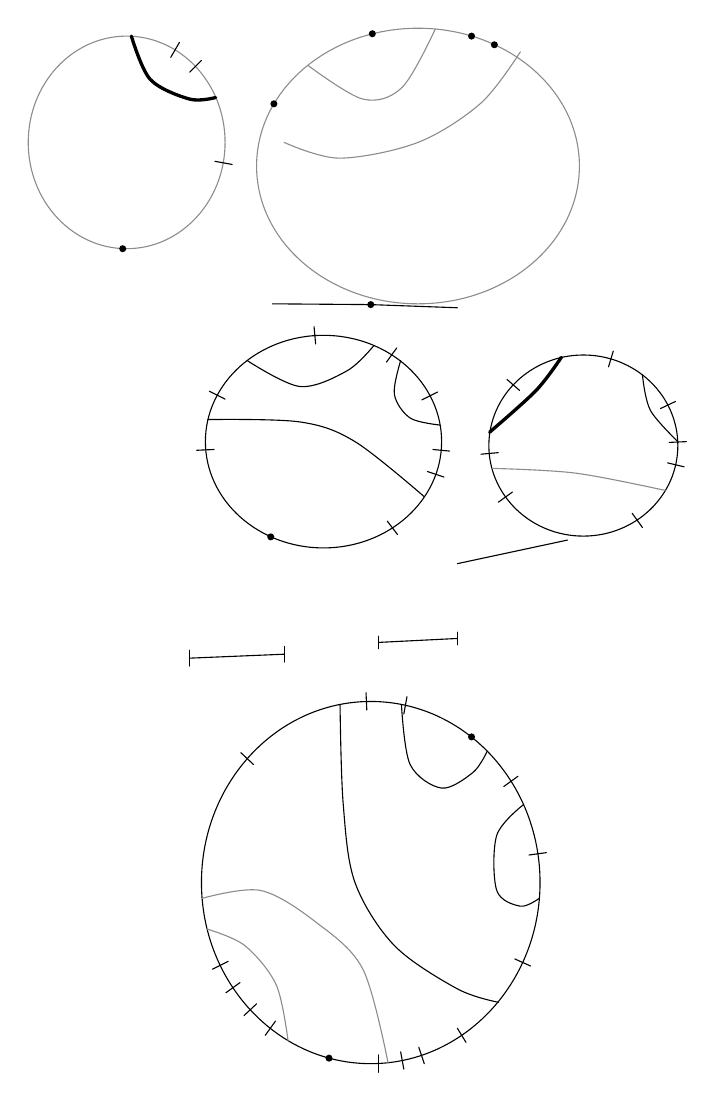
\begin{tikzpicture}[x=1mm,y=1mm,line cap=round,line join=round,font=\scriptsize]
\draw[pencil] (18,-15.7) ellipse[x radius=12.5, y radius=13.5];
\draw (23.6,-4.9) -- (24.7,-3);
\draw (26,-6.8) -- (27.5,-5.3);
\draw (29.2,-18.1) -- (31.4,-18.5);
\node[pt] at (17.5,-29.2) {};
\draw[very thick] plot[smooth, tension=0.55] coordinates {(18.6,-2.2) (21,-7.7) (26,-10.2) (29.3,-10)};
\draw[pencil] (55,-18.7) ellipse[x radius=20.5, y radius=17.5];
\node[pt] at (49.2,-1.9) {};
\node[pt] at (61.8,-2.2) {};
\node[pt] at (64.7,-3.3) {};
\node[pt] at (36.7,-10.8) {};
\draw[pencil] plot[smooth, tension=0.55] coordinates {(38,-15.7) (45,-17.7) (55,-15.7) (63,-10.7) (68,-4.2)};
\draw[pencil] plot[smooth, tension=0.55] coordinates {(41,-5.9) (48,-10.2) (53,-8.7) (57.2,-1.3)};
\draw (36.5,-36.2) -- (49,-36.3) -- (60,-36.7);
\node[pt] at (49,-36.3) {};
\draw (43,-53.7) ellipse[x radius=15, y radius=13.5];
\draw (42,-41.3) -- (41.8,-39.1);
\draw (51,-43.6) -- (52.3,-41.8);
\draw (30.5,-48.3) -- (28.5,-47.3);
\draw (29.1,-54.7) -- (26.9,-54.8);
\draw (55.5,-48.4) -- (57.5,-47.4);
\draw (56.9,-54.7) -- (59,-54.9);
\draw (56.2,-57.5) -- (58.3,-58.2);
\draw (51.1,-63.8) -- (52.4,-65.5);
\node[pt] at (36.3,-65.8) {};
\draw plot[smooth, tension=0.55] coordinates {(33.3,-43.4) (40,-46.7) (46,-44.7) (49.4,-41.5)};
\draw plot[smooth, tension=0.55] coordinates {(28.3,-50.9) (40,-51.2) (47,-53.7) (55.8,-60.7)};
\draw plot[smooth, tension=0.55] coordinates {(52.8,-43.4) (52,-47.7) (54,-50.7) (57.8,-51.6)};
\draw (76,-54.2) ellipse[x radius=12, y radius=11.5];
\draw (79.2,-44.2) -- (79.8,-42.2);
\draw (67.9,-47.2) -- (66.3,-45.8);
\draw (85.8,-49.5) -- (87.7,-48.6);
\draw (86.9,-53.8) -- (89.1,-53.7);
\draw (86.7,-56.4) -- (88.8,-56.9);
\draw (65.2,-55.1) -- (63,-55.3);
\draw (67,-60.1) -- (65.2,-61.4);
\draw (82.2,-62.8) -- (83.5,-64.6);
\draw[very thick] plot[smooth, tension=0.55] coordinates {(64.1,-52.5) (70,-47.2) (73.2,-43)};
\draw plot[smooth, tension=0.55] coordinates {(83.5,-45.2) (84.5,-49.7) (88,-53.7)};
\draw[pencil] plot[smooth, tension=0.55] coordinates {(64.4,-57.1) (75,-57.7) (86.4,-59.9)};
\draw (60,-69.2) -- (74,-66.2);
\draw (26,-81.2) -- (38,-80.7);
\draw (26,-80.2) -- (26,-82.2);
\draw (38,-79.7) -- (38,-81.7);
\draw (50,-79.2) -- (60,-78.7);
\draw (50,-78.4) -- (50,-80);
\draw (60,-77.9) -- (60,-79.5);
\draw (49,-109.7) ellipse[x radius=21.5, y radius=23];
\draw (48.5,-87.8) -- (48.4,-85.6);
\draw (53.2,-88.3) -- (53.6,-86.1);
\draw (65.9,-97.5) -- (67.7,-96.2);
\draw (34.1,-94.7) -- (32.5,-93.2);
\draw (69.1,-106.2) -- (71.3,-105.9);
\draw (67.3,-119.4) -- (69.3,-120.3);
\draw (60,-128.2) -- (61.1,-130);
\draw (50,-131.6) -- (50,-133.8);
\draw (52.8,-131.2) -- (53.2,-133.4);
\draw (55.1,-130.6) -- (55.8,-132.7);
\draw (30.9,-119.7) -- (28.9,-120.7);
\draw (32.4,-122.4) -- (30.6,-123.7);
\draw (34.5,-125.1) -- (32.9,-126.6);
\draw (36.9,-127.3) -- (35.6,-129.1);
\node[pt] at (61.8,-91.2) {};
\node[pt] at (43.7,-132) {};
\draw plot[smooth, tension=0.55] coordinates {(45.1,-87.1) (45.5,-99.7) (47,-109.7) (52,-117.7) (60,-123.2) (65.2,-124.9)};
\draw plot[smooth, tension=0.55] coordinates {(52.9,-87.1) (54,-94.7) (58,-97.7) (62,-95.7) (63.8,-93)};
\draw plot[smooth, tension=0.55] coordinates {(68.4,-99.8) (65,-103.7) (65,-110.7) (68,-112.7) (70.4,-111.7)};
\draw[pencil] plot[smooth, tension=0.55] coordinates {(27.6,-111.7) (35,-110.7) (42,-114.7) (48,-120.7) (51.2,-132.6)};
\draw[pencil] plot[smooth, tension=0.55] coordinates {(28.2,-115.6) (33,-117.7) (37,-122.7) (38.5,-129.8)};
\end{tikzpicture}
\end{document}
